% !TeX root = ../thuthesis-example.tex

\chapter{PERFORMANCE TESTING AND USABILITY EVALUATION OF VR-IOT RESEARCH PLATFORM}


План части: используем пресет из предыдущей части: лампа сяоми. Далее можем добавить пылесос в качестве примера и мобильный телефон. для каждого из них автоматически создается виртуальный объект, у всех у них хранится локация.

Для лампы добавляется новая функция - жестовое управление. Для поддержки управления жестами добавляется виртуальная камера (через тэг в опенхабе).

еще можно показать, как управлять пылесосом используя жест, указывающий на точку на полу + голосовое управление.

Дальше показывается, как это все тестируется на мак мини и на окулусе.

Замеры времени работы добавляю. Помимо этого показаны результаты тестирования на одновременную работу и соотв ошибки:
1. Объясняется, как избежать шторма запросов через рест апи и как это влияет на hci компоненту. Например, движение рук.
2. Показаны проблемы с производительностью при нескольких источниках света, и как это можно избежать с помощью внешнего сервера для вычислений.
3. Объясняются физические ограничения, можно привести ссылку на книгу о звуке.

Далее я говорю, что в этой части были расписаны именно хардварные ограничения, которы е в скором времени будут обойдены с помощью, во-первых, увеличения производительности самих устройств, а во-вторых, увеличения пропускной способности сотовых сетей, позволяющих передавать большие объемы данных за секунду, т.е. 6G, что позволит перевести большинство изменений на сервер/в облако (здесь цитирую iot в облаках статью).


TEXT STARTS HERE

Как сказано в предыдущей главе, сначала будет рассмотрен пример работы платформы, будут произведены замеры производительности.

In this chapter a smart home, one of the most common IoT environments, is used for research creating a device of a new type. The are several devices in the example configuration(link to figure = photo): 
\begin{enumerate}
    \item A Smart Wi-Fi lamp;
    \item A PC running openHAB server and NUIX-Studio App instance;
    \item A PC running NUIX-Studio App instance;
    \item An Oculus Quest VR Headset;
    \item A smart vacuum cleaner\footnote{This device will be use.}.
\end{enumerate}

The example research is on adding gesture control functionality for the smart lamp.

The virtual environment provides Widgets for Light and Gesture Recognition. In other words, a virtual lamp should be equivalent to the real-world one and gesture interface should be implemented.

\section{Server setup}
Firstly, a binding needs to be added to the openHAB server. Xiaomi Mi IO binding makes it possible to automatically add the Xiaomi Smart Wi-Fi Lamp to the server (Figure~\ref{fig:ServerSetupProcedure-figure}).

\begin{figure}
  \centering
  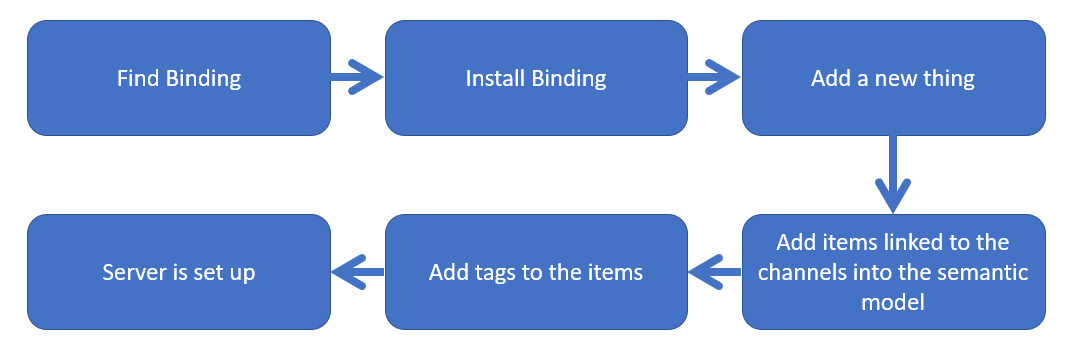
\includegraphics[width=0.9\linewidth]{figures/ServerSetupProcedure.png}
  \caption{Server setup procedure.}
  \label{fig:ServerSetupProcedure-figure}
\end{figure}

Next is adding items linked to the lamp channels. In the example the lamp brightness dimmer is added to the semantic model.

\begin{figure}
  \centering
  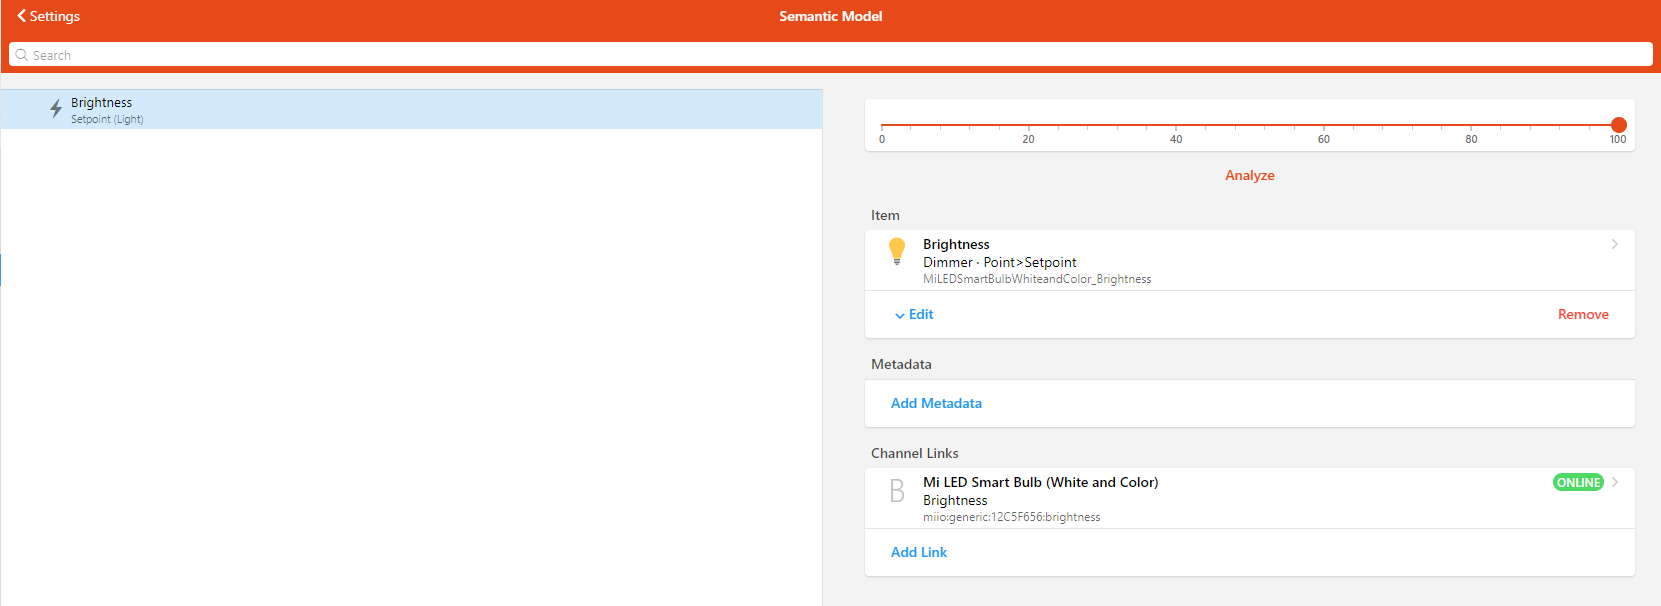
\includegraphics[width=0.9\linewidth]{figures/SemanticModelOne.png}
  \caption{Semantic model 1.}
  \label{fig:SemanticModelOne-figure}
\end{figure}

As seen in Figure~\ref{fig:SemanticModelOne-figure}, the brightness can be already controlled by moving the dimmer. The real-world lamp will change the brightness based on the value on the server.

Next step is adding tags to the item: the lamp should be controlled by Gestures, then a corresponding tag has to be added (Figure~\ref{fig:ItemEditPage-figure}).

\begin{figure}
  \centering
  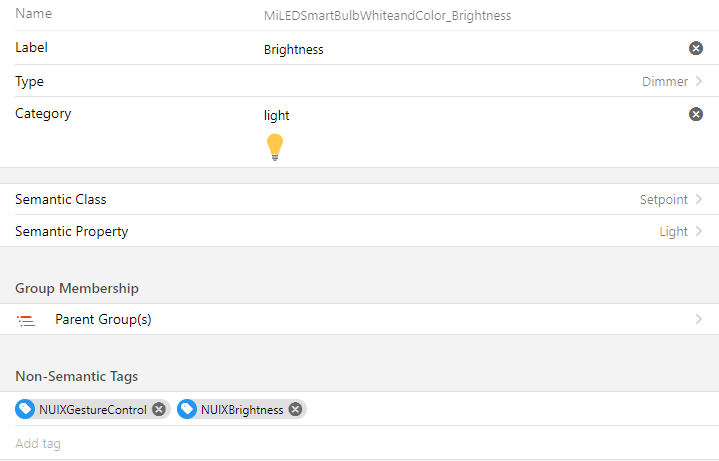
\includegraphics[width=0.9\linewidth]{figures/ItemEditPage.png}
  \caption{Item Edit Page.}
  \label{fig:ItemEditPage-figure}
\end{figure}

The server has been set up.

\section{Running NUIX-Studio APP}

After the server has been set up, and the environment has been chosen the platform is ready to run on the devices.

\section{Performance analysis}

Анализ производительности платформы не является основной целью исследования, но тем не менее, он показателен с точки зрения нахождения бутылочных горлышек. Будет показано, что задачи рендеринга имеет смысл выполнять на отдельном сервере, а иметь общую базу данных для всех экземпляров приложения поможет добиться в итоге одновременной работы нескольких пользователей внутри системы.


Тест 1: запуск одного источника света на окулусе с хорошей четкостью. Фпс падает до 20, невозможность нормально перемещаться по комнате и управлять светом. Переносим обработку света на сервер. Теперь фпс на окулусе уже 72, и можно выполнять считывание рук с большей частотой. Таким образом, и яркость лампы на сервере меняется чаще. 

обобщение в конце главы.

Тест 2: Одновременная работа нескольких устройств. Так как устройства работают в одной вай-фай сети через рест апи, минимальное время синхронизации между экземплярами приложения составляет время передачи сигнала от одного устройства к другому. Замеряем его: получаем какое-то значение (от мака к ноуту + от ноута к окулусу - т е от мака к окулусу и обратно). теперь делаем замер через изменение яркости лампы на маке. Двигвем ползунок - отправился на сервер, с сервера отправилось всем устройствам, а внутри окулуса произошло изменение ползунка и яркости. далее от него может пойти в обратную сторону, и тут мы замеряем, когюа на мак приходит ивент с отправленным значением (но он скипается, потому что значение то же). Видим, что разница мизерная. Помимо этого, необходимо добавить погрешность рендеринга. Соответственно, совместная работа в реальном времени возможна.

Тест 3: Можно проверить появление устройства в реальном времени. Типа добавляем пылесос, и на сколько быстро он появляется на эпп инстансе. Опять же, ограничено лишь сетью.

Дальнейшее тестирование не проводилось, так как прототип платформы в таком не нуждается, вот.


Теперь по поводу удобства использования. Различные баги:

существует много проблем:

вирутальная клавиатура, пропадающие руки.




The first experiment is the analysis of the system startup, performed on three devices by registering the startup time (Figure~\ref{fig:SystemStartupScheme-figure}).

\begin{figure}
  \centering
  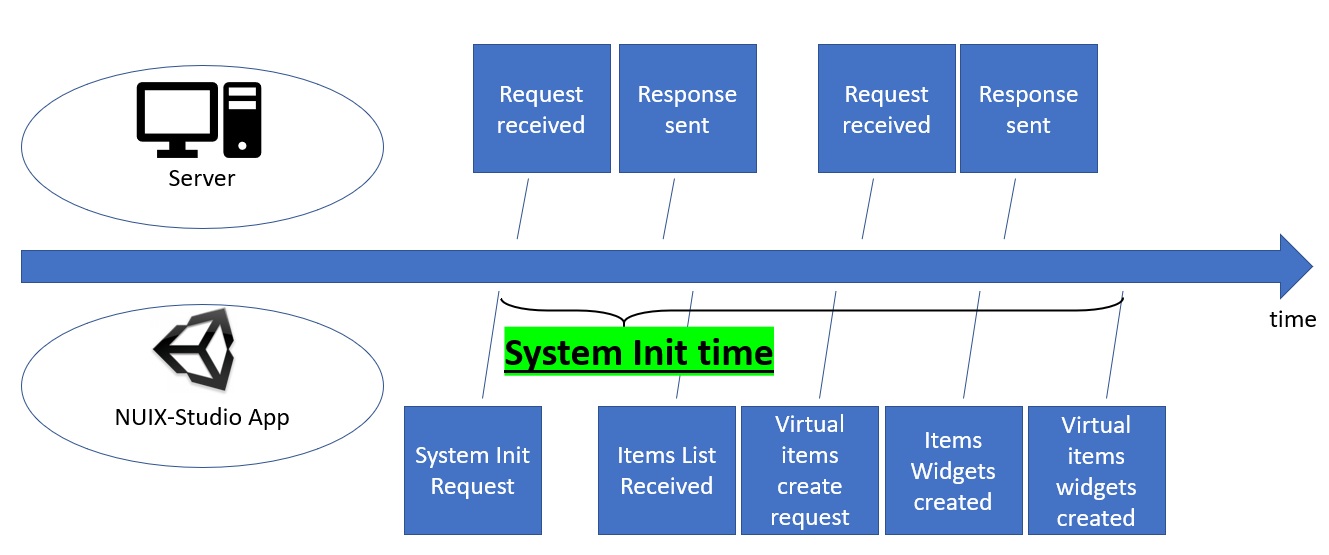
\includegraphics[width=0.9\linewidth]{figures/SystemStartupScheme.png}
  \caption{System startup scheme.}
  \label{fig:SystemStartupScheme-figure}
\end{figure}

The hardware specifications can be seen on Table~\ref{tab:hardware-specifications-table} \footnote{Localhost PC is a notebook running openHAB server as well as one instance of NUIX-Studio APP; Remote PC is a computer running one instance of NUIX-Studio APP and connected to the same Wi-Fi network as localhost PC; Oculus Quest is a Virtual Reality Headset running NUIX-Studio APP and connected to the same Wi-Fi network as PCs.}.

\begin{table}
  \centering
  \begin{threeparttable}[c]
    \caption{Hardware specifications in the experimental setup}
    \label{tab:hardware-specifications-table}
    \begin{tabular}{ll}
      \toprule
      Unit    &         Specifications                 \\
      \midrule
      Localhost PC & Ryzen 5 3500u, Windows 10 \\
      Remote PC & Core i5 4278U, macOS 11.2.3    \\
      Oculus Quest        & Qualcomm Snapdragon 835, Android-based            \\
      \bottomrule
    \end{tabular}
  \end{threeparttable}
\end{table}

Each test was performed on a new instance of Unity APP to avoid cashing influence. And then mean values have been calculated (Figure~\ref{fig:SystemInitTime-figure}).

\begin{figure}
  \centering
  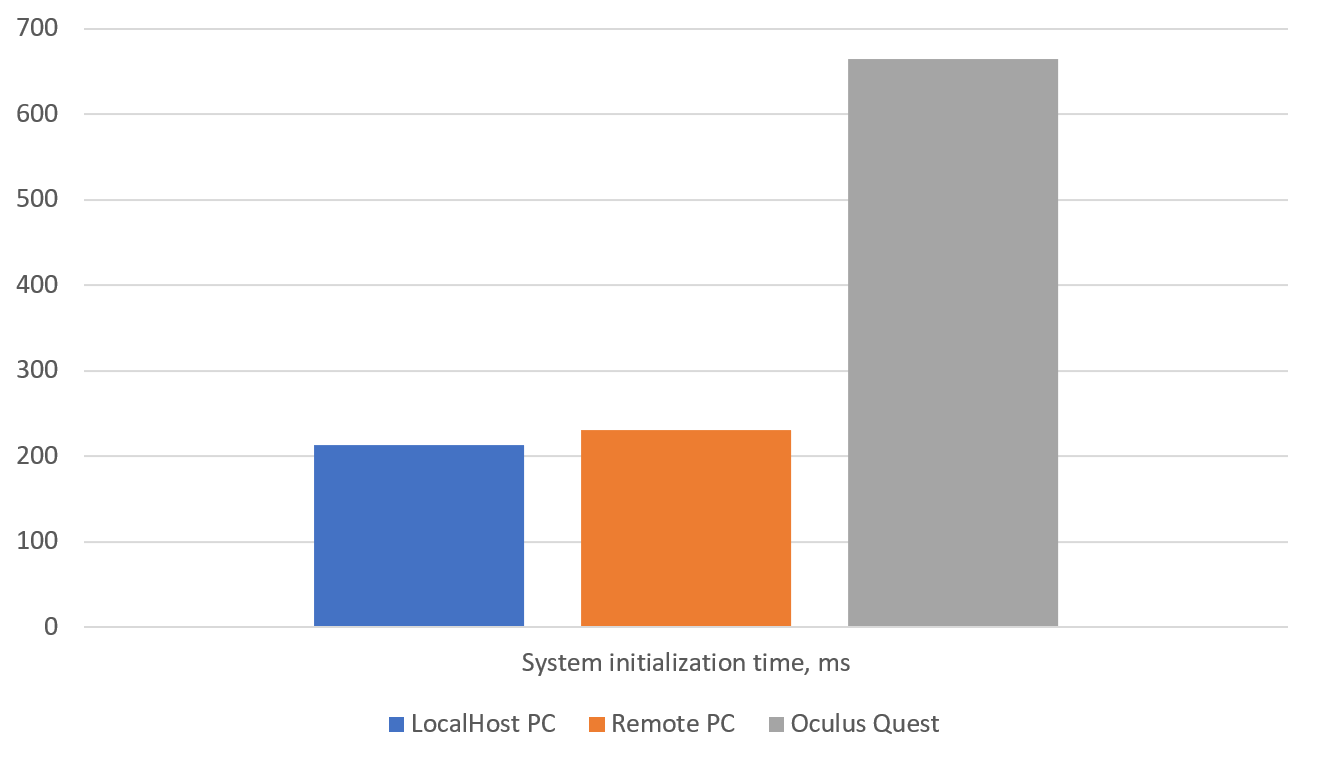
\includegraphics[width=0.9\linewidth]{figures/SystemInitTime.png}
  \caption{System initialization time measured on different client devices.}
  \label{fig:SystemInitTime-figure}
\end{figure}

As seen on Figure~\ref{fig:SystemInitTime-figure}, the system initialization time is a time-consuming operation, which from 200 to over 600ms in average to perform.


